%!TEX root = draft.tex
\section{Overview}
\label{sec:overview}

% \gpnote[inline, nomargin]{Add an intuitive notion of history.}
% (adapted from~\cite{ShapiroPBZ11})
\begin{figure}[t]
\begin{lstlisting}[basicstyle=\ttfamily\scriptsize,caption={Replicated Growing Array (RGA) CRDT pseudo-code.},captionpos=b,label={lst:rga}]
  payload Ti-Tree N, Set Tomb
  initial N = @|$\emptyset$|@, Tomb = @|$\emptyset$|@
  //@ initial lin = @|$\epsilon$|@

  addAfter(a,b) :
    atSource :
      precondition : a = @|$\circ$|@ or (a != @|$\circ$|@ and (a,_,_) @|$\in$|@ N and a @|$\not\in$|@ Tomb)
      let ts@|$_{\mathtt{b}}$|@ = getTimestamp()
      //@ lin = insert(lin, addAfter(a,b), ts@|$_{\mathtt{b}}$|@)
    downStream(a, ts@|$_{\mathtt{b}}$|@, b) :
      N = N @|$\cup$|@ {(a, ts@|$_{\mathtt{b}}$|@, b)}
      //@ N' = N @|$\cup$|@ {(a, ts@|$_{\mathtt{b}}$|@, b)}

  remove(a) :
    atSource :
      precondition : (a,_,_) @|$\in$|@ N and a @|$\notin$|@ Tomb
      //@ lin = insert(lin, remove(a), max(@|$\{\tsof(\alabel)\ |\ \alabel\in \alabelset\}$|@))
    downStream(a) :
      Tomb = Tomb @|$\cup$|@ {a}
      //@ Tomb' = Tomb @|$\cup$|@ {a}

  read() :
    let ret-list = traverse(N, Tomb)
    //@ lin = insert(lin, read()@|$\Rightarrow$|@ret-list, max(@|$\{\tsof(\alabel)\ |\ \alabel\in \alabelset\}$|@))
    return ret-list
\end{lstlisting}
\end{figure}

We give an informal description of the system model
we assume, and illustrate our main contribution with two
interesting CRDT implementations extracted from~\cite{AttiyaBGMYZ16,ShapiroPBZ11}.

\subsection{System Model}
\label{sec:sys-model}
<<<<<<< HEAD
\begin{wrapfigure}{r}{0.5\textwidth}
  \centering
  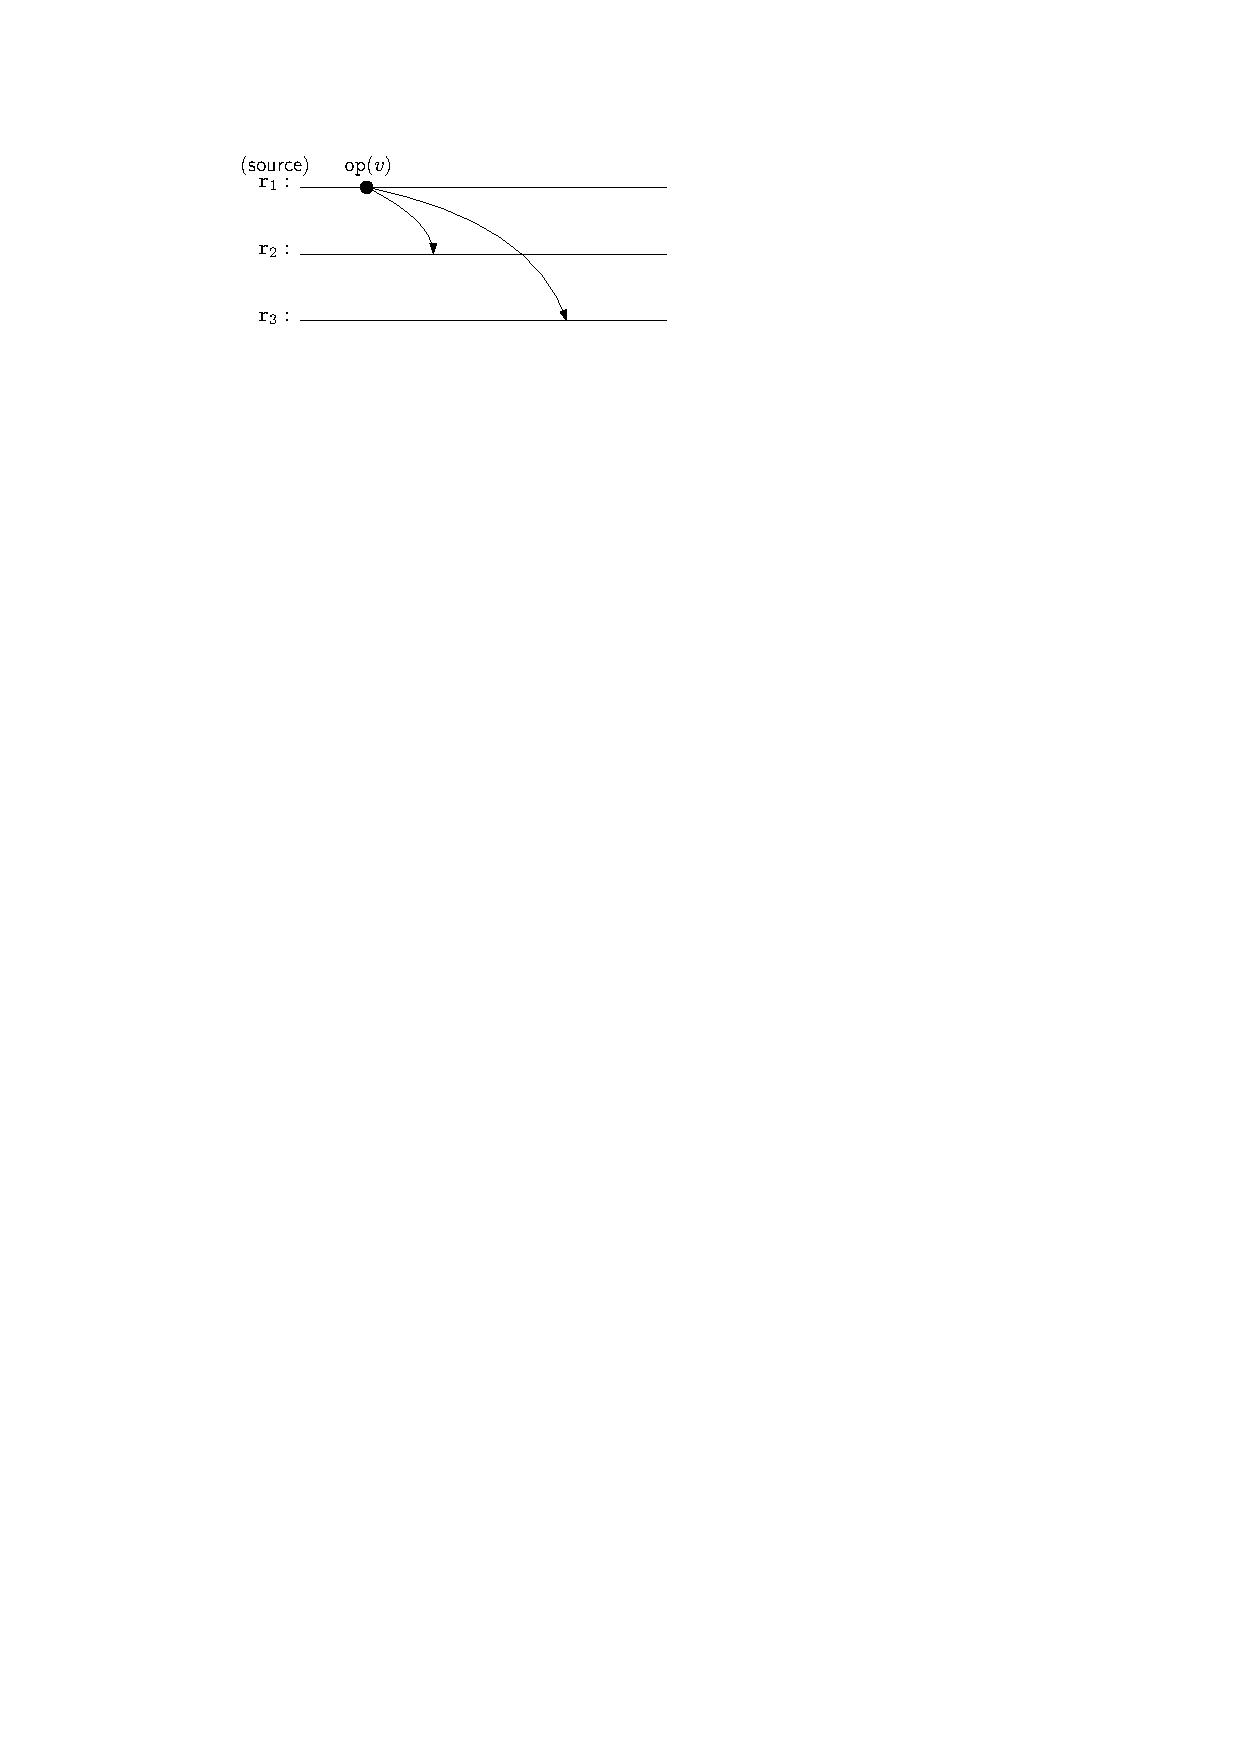
\includegraphics[scale=.9]{figures/sys-mod}
  % \vspace{-20pt}
=======

\begin{wrapfigure}{r}{0.42\textwidth}
\vspace{-4mm}
  \centering
  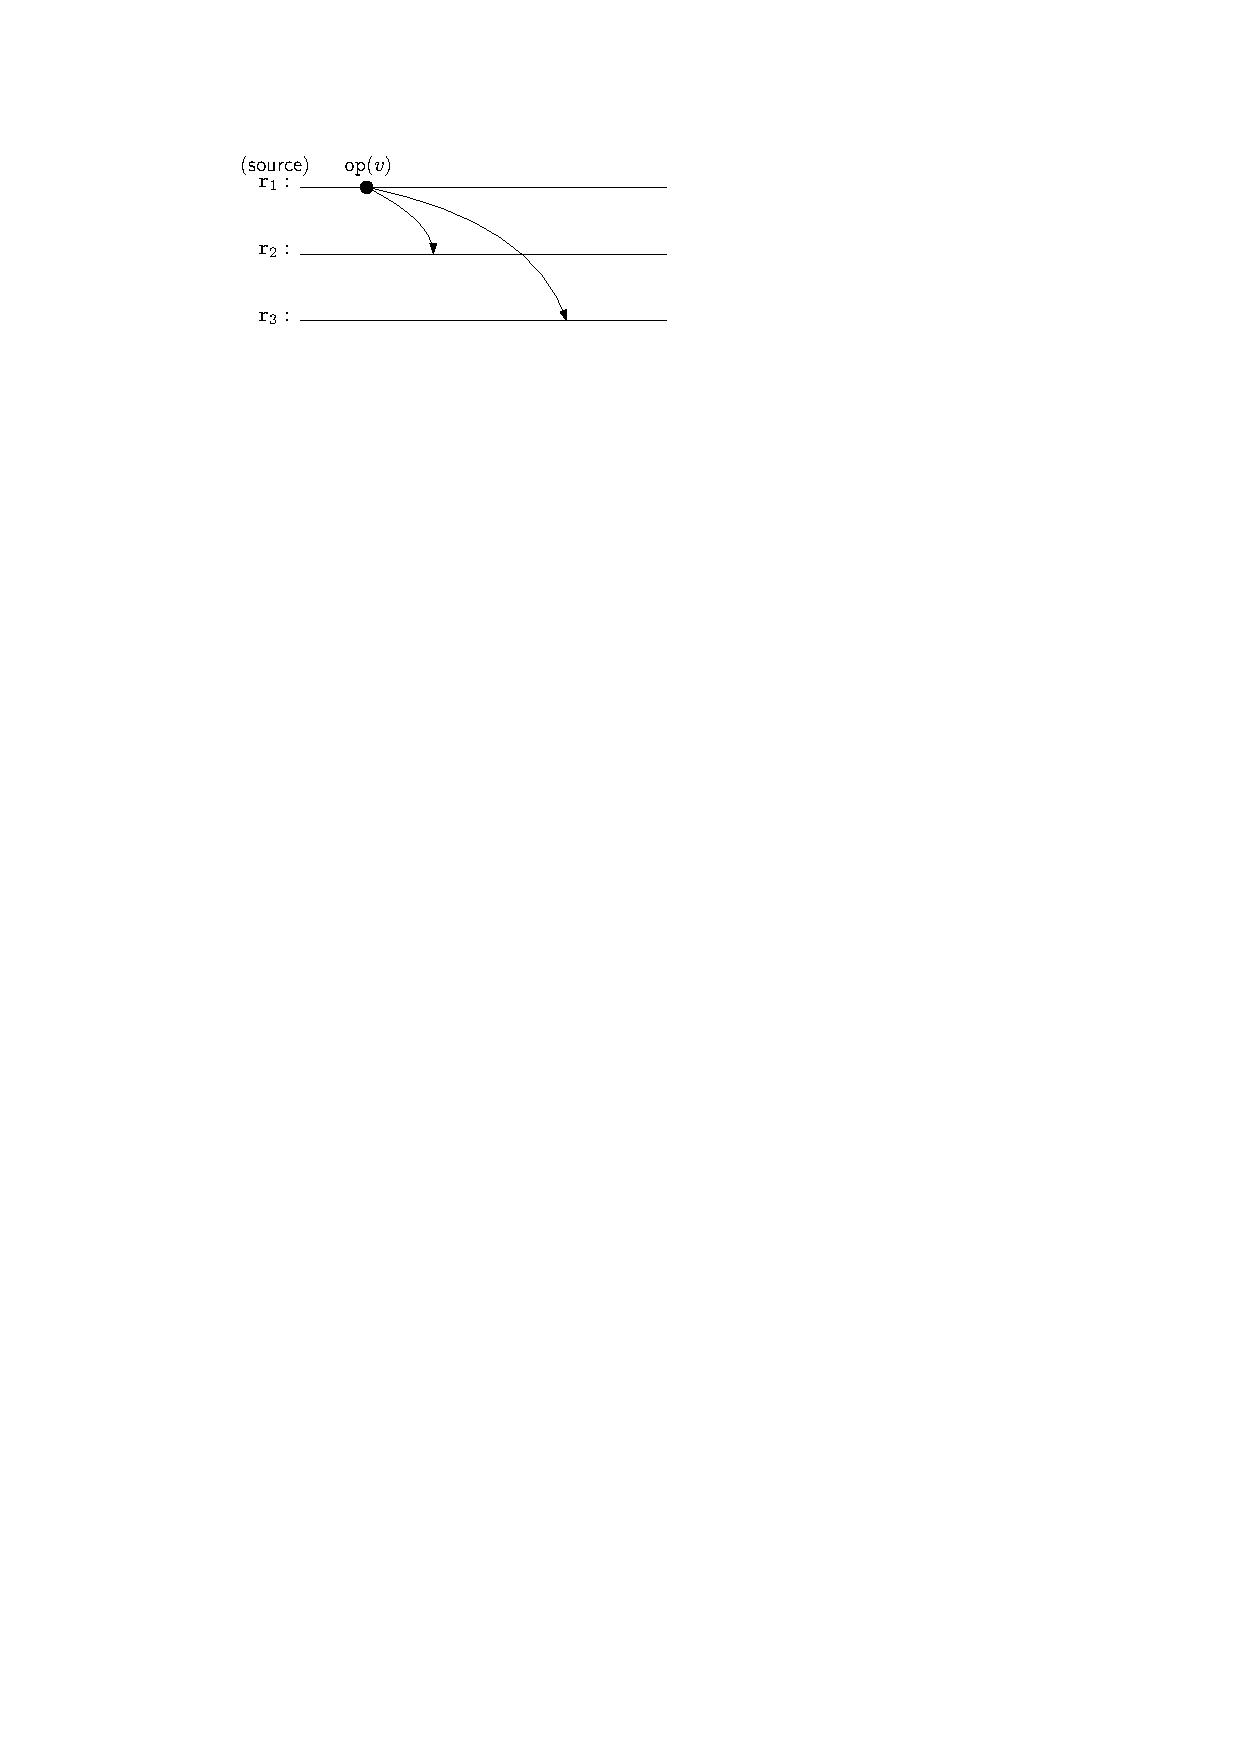
\includegraphics[scale=.7]{figures/sys-mod}
>>>>>>> origin/master
  \caption{CRDT System Model.}
  % \vspace{-20pt}
  \label{fig:sys-mod}
\end{wrapfigure}
We assume that the system is comprised of multiple nodes in a network.
In this work we will be concerned with the implementation of CRDTs,
and we will usually concentrate our discussion to the behaviors
allowed for \emph{an instance} of the data type.
We will generically call such an instance an \emph{object}.
As mentioned in Section~\ref{sec:introduction} we assume that objects are
replicated among the participating nodes of the system -- called replicas.

% \gpwarning{Redraw pictures.}
% on a replicated object
The execution model for an operation \lstinline|op(v)| is depicted in Figure~\ref{fig:sys-mod} and it proceeds as follows:
\begin{itemize}
\item A client, i.e., a program issuing calls to the object, connects
  to any one replica %(a node of the system holding a copy of the object)
  and performs the operation in that replica. We call such a
  replica the source or \emph{origin}. The source of \lstinline|op(v)|
  in Figure~\ref{fig:sys-mod} is the replica $\arep_1$ on the top.
  Then, executing an operation is done in two phases.
\item Assuming that the operation requires reading and updating the
  state of the object, the state of the object in the origin replica is
  read first.
  We shall sometimes refer to this part of the operation as the
  \emph{generator} following~\cite{ShapiroPBZ11}.
  Then, if the state needs to be changed as part of the operation --
  e.g. an \lstinline|addAfter| operation of RGA -- an update is
  generated which shall be executed in all the replicas holding copies of the
  object.
  We shall refer to the update as the \emph{effector}.
  We assume throughout this paper that effectors are executed
  immediately at the origin replica.
  This is represented by the dot at the origin replica
  in Figure~\ref{fig:sys-mod}.
\item Finally, as the system progresses, the effector of the operation
  will be delivered to each of the replicas holding a copy of the
  object, and the state of each of the replicas will be updated
  consequently.
  This is represented by the target of the arrows
  in Figure~\ref{fig:sys-mod}.
\end{itemize}
% This model is depicted in~\autoref{fig:system-model}.
% \fxwarning[nomargin, inline]{We need the picture}.

%\smallskip
\noindent
{\bf CRDT implementations.}
We write the code of CRDT implementations using the syntax introduced in \citet{ShapiroPBZ11}.
%Following the description above, \citet{ShapiroPBZ11} present the code
%of a number of CRDT implementations.
%
For instance, Listing~\ref{lst:rga} shows the code of the RGA algorithm, 
where the lines starting with \lstinline|//@| should be ignored for the moment 
(this is a version of the RGA algorithm introduced in~\cite{AttiyaBGMYZ16}
which we believe is simpler to understand).
%
Let us first consider the structure of the data type implementation:
\begin{itemize}
\item The keyword \lstinline|payload| introduces the state that is
  used to represent the object. This is akin to the fields of a class
  in an object oriented language such as Java. In the
  case of RGA we have a variable \lstinline|N| of type
  \lstinline|Ti-Tree| (to be discussed later), and a variable
  \lstinline|Tomb| of type \lstinline|Set|.
\item After that we find the definitions of the three operations we
  discussed in the introduction: \lstinline|addAfter|,
  \lstinline|remove| and \lstinline|read|.
\item The effectful operations \lstinline|addAfter| and
  \lstinline|remove| have two labels marked in red:
  \lstinline|atSource| and \lstinline|downStream|.
  These represent the code to be executed as the generator and
  effector respectively. Hence, the code under the label
  \lstinline|atSource| is executed only at the origin replica and it
  generates the arguments that the code under \lstinline|downStream|
  will execute in each of the replicas (including the origin).
\item The 
  \lstinline|precondition| annotations indicate facts that are
  assumed about the state of the object upon execution of either of
  the generator or effector of the operation.
\end{itemize}
Reconsidering Figure~\ref{fig:sys-mod} the
source of the arrows in a replica represents the execution of an
\lstinline|atSource| jointly with the \lstinline|downStream| of the
operation at the origin replica.
%
The target of the arrows represents the delivery and execution of the
effector of the operation in a replica other than the origin.


In the rest of this section we consider two examples of CRDT
implementations and their RA-linearization arguments.

\subsection{RGA CRDT Implementation}
\label{sec:rga-crdt-impl}

% \paragraph{RGA CRDT implementation}
As it is common to many CRDT implementations, RGA replicas will use
a timestamp mechanism to keep track of the causality between updates
to the list, effectively capturing when two updates are concurrent.
Moreover, they will keep the information relating the causal order
in which elements are added to the list.
%
Provided with this causality information -- or lack thereof--, the
timestamps will be used to resolve conflicts in a deterministic way.
%
More concretely, each replica will keep what we shall name a
\emph{Timestamp Tree} (\lstinline|Ti-Tree|) containing in every tree
node a pair with: the element added to the list (for instance the
character \lstinline|b|), and a timestamp associated to it
(\lstinline|t|$_{\mathtt{b}}$) used to resolve conflicts.
%
We will encode the tree as a set containing triples (corresponding to
nodes) of the form (\lstinline|a|, \lstinline|ts|$_{\mathtt{b}}$, \lstinline|b|)
representing the fact that there is an element \lstinline|b| in the
tree with timestamp \lstinline|ts|$_{\mathtt{b}}$ and whose parent is
the item \lstinline|a| also present in the tree.
%
The tree-ness property is ensured by construction.


% \begin{wrapfigure}{l}{.3\textwidth}
%   \centering
%   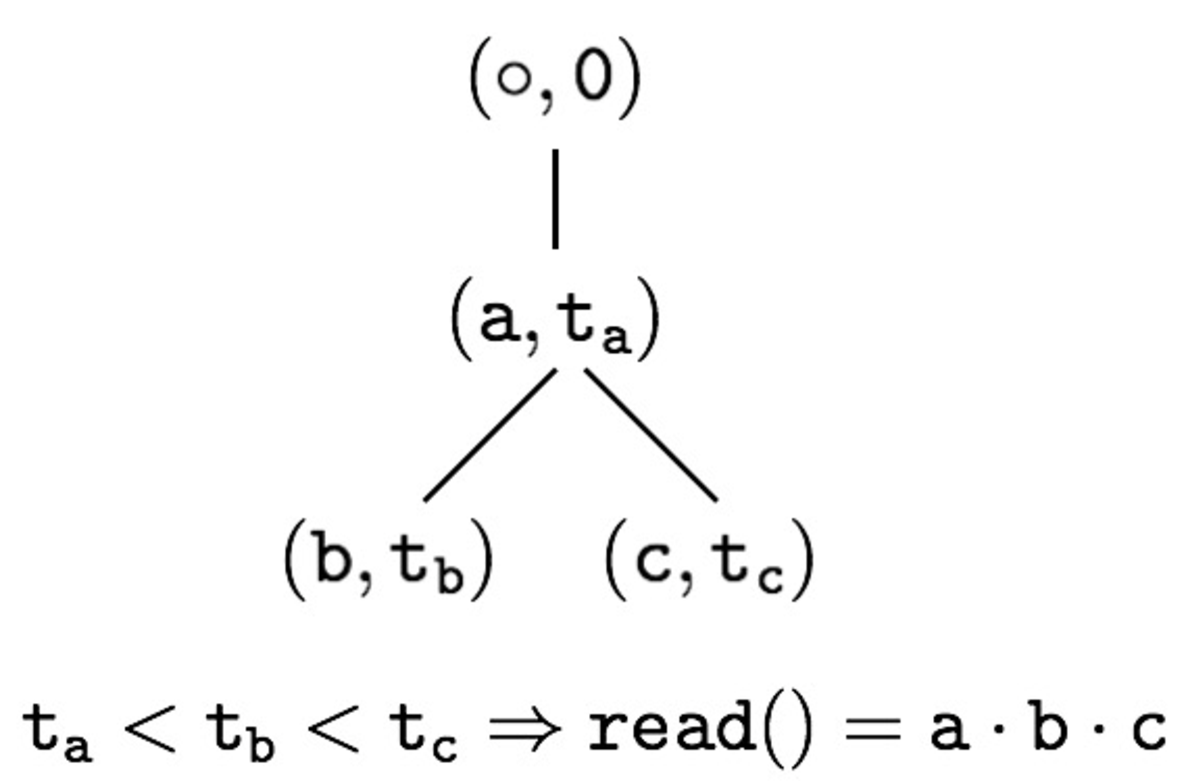
\includegraphics[scale=.9]{figures/simple-ti-tree}
%   \caption{RGA Ti-tree example.}
%   \label{fig:rga-tree}
% \end{wrapfigure}
If we look at the \lstinline|atSource| portion of the
\lstinline|addAfter(a,b)| method we can see that the precondition requires
the element \lstinline|a| to exist in the tree before the insertion of
\lstinline|b| after it.
%
We remark at this point that the data structure is initialized with a
preexisting initial element denoted by $\circ$.
%
The generator then samples a timestamp \lstinline|t|$_{\mathtt{b}}$
for \lstinline|b| which is assumed to be larger than any
timestamp presently occurring in the \lstinline|Ti-Tree|
\lstinline|N| of the origin replica~\footnote{Also, \lstinline|t|$_{\mathtt{b}}$ cannot 
be sampled by another replica invoking \lstinline|addAfter| (as we discussed
in Section~\ref{sec:introduction} this can be ensured by tagging the timestamps with replica identifiers).}.
%
Looking at the \lstinline|downStream| portion of
\lstinline|addAfter(a,b)| we see that the effect of the operation is
to add the triple \lstinline|(a, ts|$_{\mathtt{b}}$\lstinline|, b)|
in the replica's own copy of \lstinline|N|.
%
This ensures that the tree structure is consistent with the causality
of insertions in the data structure.
%
Notice that a client of the object will only ever attempt to add an
element after another element which it has already seen as mandated by
the \lstinline|addAfter| API.
%
Hence, the parent node of any node was inserted before it, and is
causally related to it.
%
Similarly, nodes that are not related to each other on any path of
the tree (eg. siblings) are not causally related.
% \footnote{The converse
%   is not true. There can be nodes that are linked by ancestry in the
%   tree resulting from concurrent operations, but this does not affect
%   the correctness of the algorithm.}
%
An example of such a tree is shown in the left most box
of Figure~\ref{fig:rga-trace}, where we can see that
elements \lstinline|c| and \lstinline|b| were concurrently added after
\lstinline|a|, and \lstinline|a| was added first after the
initialization element $\circ$.

Considering a \lstinline|Ti-tree| constructed in this way, we can
obtain a list by traversing the tree in pre-order fashion, with the
proviso that siblings are ordered according to their timestamps with
the \emph{highest timestamp visited first}.
%
Again, the leftmost box in Figure~\ref{fig:rga-trace} shows a tree that
results in the list $\mathtt{a \cdot b \cdot c}$ assuming that the
timestamp order is $\mathtt{ts_a < ts_c < ts_b}$.

\begin{figure}[t]
  \centering
  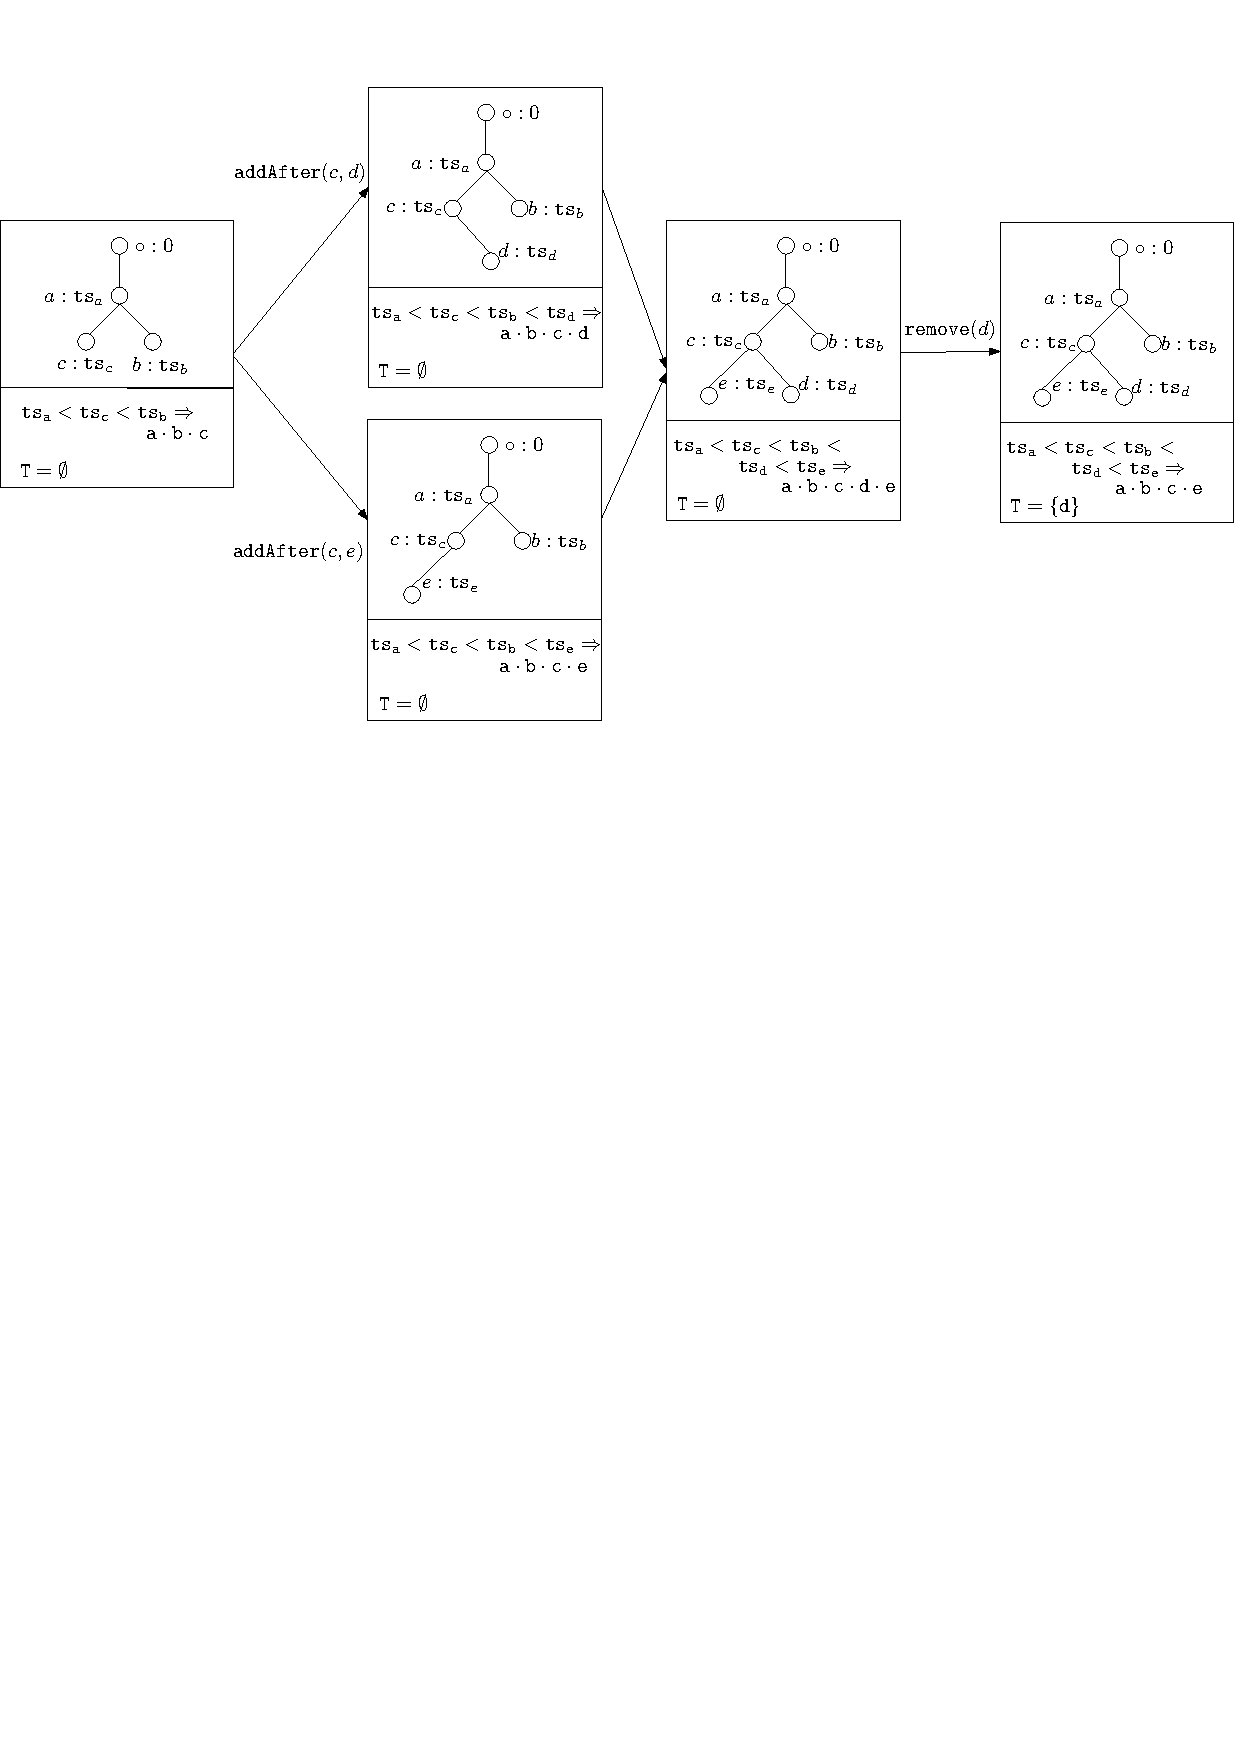
\includegraphics[width=.8\textwidth]{figures/RGA-Trace}
% \vspace{-10pt}
  \caption{Example of RGA conflict resolution.}
  \label{fig:rga-trace}
\end{figure}

Let us now consider the case of two concurrent operations:
\lstinline|addAfter(c,d)| and \lstinline|addAfter(c,e)| executing in
two different replicas starting both with the state depicted on the
left of Figure~\ref{fig:rga-trace}.
%
Following the code in Listing~\ref{lst:rga} we obtain the trees in the
second column of Figure~\ref{fig:rga-trace} where we assume that the
top tree is the result of \lstinline|addAfter(c,d)| in one of the
replicas, and the bottom tree is the result of executing
\lstinline|addAfter(c,e)| in the other replica.
%
As it can be seen, the two trees result in different lists in each
replica before the operations are mutually propagated.
%
In the third column of Figure~\ref{fig:rga-trace} we obtain the
result of propagating the operations between the replicas -- indeed
the propagation of any of the operations to any of the replicas
engenders this tree, since the result would be the same (c.f. the
commutativity of CRDT).
%
It is clear now that the result of the list is $\mathtt{a \cdot b
  \cdot c \cdot d \cdot e}$.


% \gpnote*{By Chao. Should be elsewhere}{
% \figurename~\ref{fig:how RGA works} gives a example of how RGA do conflict resolution for concurrent $addAfter$ operations, and how it do $remove$: if from one local state we do concurrent $\alabelshort[addAfter]{b,c}$ and $\alabelshort[addAfter]{b,d}$, then it converges. If we then do $\alabelshort[remove]{b}$, we just add $b$ into tombstone. Here we assume $\ats_a$, $\ats_b$, $\ats_c$ and $\ats_d$ is the timestamp of $a$, $b$, $c$ and $d$, respectively, and the timestamp order be $\ats_a < \ats_b < \ats_c < \ats_d$.
% }

We have so far ignored the \lstinline|remove| operation.
%
Consider the case where a client issues an \lstinline|addAfter(a, b)|
on a replica while another client issues a \lstinline|remove(a)|
operation in another replica.
%
If the effector of \lstinline|remove(a)| reaches every replica after
the effector of \lstinline|addAfter(a, b)| there is no problem since
the semantics is obvious, the element \lstinline|a| is removed after
the element \lstinline|b| has been added.
%
However, if the operations reach some replica in the opposite order
(recall that these are concurrent operations) we have a problem since
the precondition of the effector of \lstinline|addAfter(a, b)|
requires that the element \lstinline|a| be present in the
\lstinline|Ti-tree| of the replica.

To avoid this kind of conflict, thus rendering these operations
commutative (c.f. CRDT), RGA does not really erase elements from the
\lstinline|Ti-tree|.
%
Instead, an additional data structure called a tombstone is used to
keep track of elements that have been conceptually erased and should
not be considered when reading the data structure via \lstinline|read|.
%
In our case the tombstone is simply a set \lstinline|Tomb| of
elements.
%
With this explanation the code of the \lstinline|remove| operation
in Listing~\ref{lst:rga} should be self-explanatory.
%
The last column of Figure~\ref{fig:rga-trace} shows the result of
removing item $\mathtt{d}$ from the list.

Then, the implementation of \lstinline|read| performs the pre-order
traversal as explained before, where all the elements in the tombstone
\lstinline|Tomb| are ignored from the output list.
%
In each of the boxes of Figure~\ref{fig:rga-trace} the list shown
represents the result of a \lstinline|read| operation in the state
depicted.

% \fxwarning[nomargin, inline]{It's not clear what we are linearizing. I think we should say that standard linearizability considers the partial order given by real-time while here we consider the visibility relation}

% \fxwarning[nomargin, inline]{We should already explain the issue of queries, the fact that RGA is not linearizable in the classical sense.}

\begin{wrapfigure}{L}{.5\linewidth}
  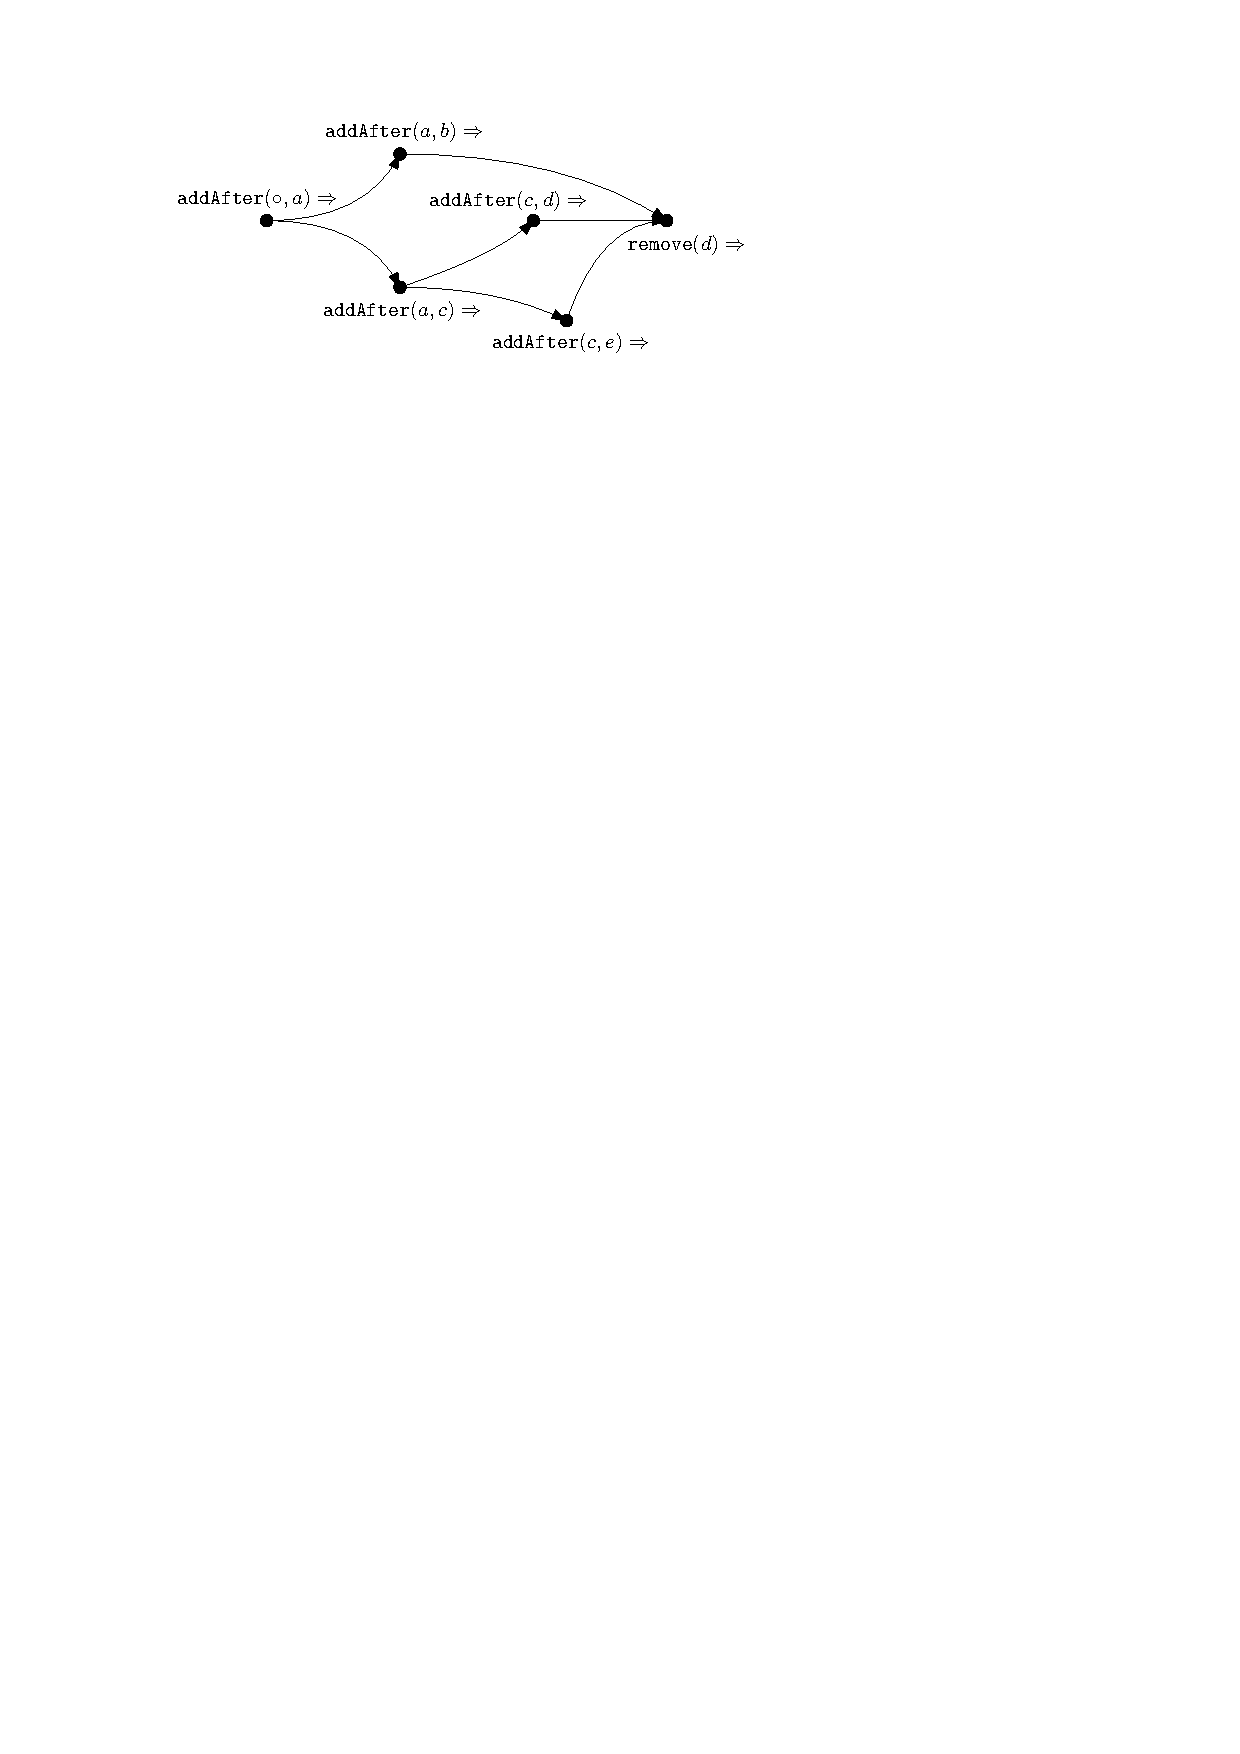
\includegraphics[scale=.7]{figures/history-RGA}
  \caption{A history for the RGA object.}
  \label{fig:rga-history}
\end{wrapfigure}

\smallskip
\noindent
{\bf Operations, histories and linearizability.}
Let us now consider a more abstract view of executions of a 
CRDT object called \emph{history}.
%
Informally a history is a set of operations with a partial order
representing the ordering constraints imposed on the execution of each
of the operations.
%
We will represent the execution of an operation with a label of the
form $\alabellong{\argv}{\retv}$ representing a call to method
$\amethod$ with arguments $\argv$ and whose return value is $\retv$.
%
When the values are unimportant we shall use the meta-variable
$\alabel$ to denote a label~\footnote{We can assume here that each of these labels is uniquely identified.}.
%
The partial order mentioned above represents the \emph{visibility} relation among operations, where we say that an
operation with label $\alabel_1$ is visible to another operation with
label $\alabel_2$ if at the time when $\alabel_2$ was first executed
at the origin replica, the effects of $\alabel_1$ where incorporated
in the state of the replica executing $\alabel_2$.
%
Then, a history is a pair $(\alabelset, \prec)$ containing a
set of labels $\alabelset$ and a visibility relation $\prec$ between labels. 
%incorporating the constraints enforced by the execution.
%
For instance, the history %where the constraints are given by visibility
corresponding to the execution in Figure~\ref{fig:rga-trace} 
is presented in Figure~\ref{fig:rga-history}.
%, where we can see the
%partial order resulting from the visibility relation of the execution
%explained in~\autoref{fig:rga-trace}. 
%
Each node of the history represents a label in the set $\alabelset$
and the arrows represent that the operation corresponding to the
source is visible to the operation at the target.
%
Since we assume that the visibility is transitive we ignore
redundant arrows derivable from transitivity.

A similar notion of history is used in the context of \emph{linearizability}~\cite{HerlihyW90}, 
the de-facto correctness condition of concurrent data structures.
 % is \emph{linearizability}~\cite{HerlihyW90}.
The only difference is that the order $\prec$ relates two operations originating from the same process
as well as any two operations the first of which returns before the
other one started. Then, a history $(\alabelset, \prec)$ is called linearizable
if there exists a \emph{sequential} history $(\alabelset, \prec_{\mathsf{seq}})$ (i.e., $\prec_{\mathsf{seq}}$ is a total order of the operations in
  $\alabelset$), called \emph{linearization},
such that
\begin{inparaenum}[(i)]
\item $(\alabelset, \prec_{\mathsf{seq}})$ is a valid execution of the object, and
%\item $\prec_{\mathsf{seq}}$ is a total order of the operations in
%  $\alabelset$, and
\item $ \prec\ \subseteq\ \prec_{\mathsf{seq}}$.
\end{inparaenum}
%%
%Linearizability requires that for any execution of a concurrent
%object, there must exists an ``equivalent sequential'' (or linear)
%execution where each of the operations sees the effects of all
%operations prior to it.
%%
%The notion of equivalent here requires that the set of executed
%operations are the same -- that is the method, arguments, and return
%value of each operation are preserved.
%%
%Then, linearizability requires that whenever two operations are
%sequentially ordered by the client code executing them, they should
%appear in the linear ordering in that order.
%%
%A final constraint imposed by linearizability, sometimes referred to
%as real-time order, is that whenever an operation returns at a time
%prior the starting time of another operation (concurrent or not),
%these operations must respect this order in the linearization.
%%
%
%To make these notions precise without referring to implementation
%details we will consider \emph{execution histories}.
%%
%%
%For instance, in the case of linearizability as in~\cite{HerlihyW90}
%the order $<$ relates two operations originating from the same process
%as well as any two operations the first of which terminated before the
%other one started.
%%
%
%Then, the linearizability requirement for an execution history
%$(\alabelset, <)$ is that there exists a \emph{sequential execution}
%history $(\alabelset, <_{\mathsf{seq}})$ such that
%\begin{inparaenum}[(i)]
%\item $(\alabelset, <_{\mathsf{seq}})$ is a valid execution of the object,
%\item $<_{\mathsf{seq}}$ is a total order of the operations in
%  $\alabelset$, and
%\item $ <\ \subseteq\ <_{\mathsf{seq}}$.
%\end{inparaenum}

While linearizability is an adequate correctness criterion for
systems with strong synchronization assumptions (for instance
shared-memory systems), it is not adequate for replicated distributed
systems.
%
In the specific case of CRDTs, we need to accommodate for the fact
that operations are propagated lazily, so two replicas can see
non-coinciding sets of operations.
%
Hence we relax linearizability to adapt it to CRDTs as follows:
\begin{inparaenum}
\item we require that the sequential history be consistent with
the visibility relation among operations instead of the returns-before order, and
\item operations that only read the state of the object are allowed
to see a \emph{sub-sequence} of the linearization, instead of
the whole prefix as in the case of linearizability.
\end{inparaenum}
(We will discuss one additional relaxation in Section~\ref{sec:or-set-crdt}).
%
%Our relaxations requirethat the linear execution be consistent with
%the visibility relation among operations (instead of the returns-before order)
%%
%Hence, our notion of history instead of using the real-time order
%described above uses visibility as the underlying order of executions.
%%
%%
%For operations that only read the state of the object, we will allow
%them to see a to see a sub-sequence of the linearization, instead of
%the whole prefix as in the case of~\cite{HerlihyW90}.
%%
%
Let us now illustrate these intuitions through examples.
% %
% That is, that there exists a total order of the operations such that
% the result of each operation corresponds to the execution of all the
% operations prior to it in the order (c.f.
% linearizability~\cite{HerlihyW90}).
% %

\smallskip
\noindent
{\bf Intuition of RGA \CRDTLinshort{}.}
To simplify the argument which will be made precise in the following
section we focus first on the linearization of two concurrent
operations adding an element after a common element.
%
Let us say that we have two concurrent \lstinline|addAfter(a,b)| and
\lstinline|addAfter(a,c)| operations.
%
This example corresponds to a history formed of the first three nodes
of Figure~\ref{fig:rga-history} from left to right.
%
Because these operations are concurrent they are not related by
visibility (by definition of concurrent) so our criterion allows for
any ordering among them.
%
Can we show that these operations can always be ordered one way or
another such that the result of all subsequent reads will correspond
to this ordering?
%
In fact, from the explanation given above we know that the order
between \lstinline|b| and \lstinline|c| in the resulting list will be
determined by their corresponding timestamps
(\lstinline|t|$_{\mathtt{b}}$ and \lstinline|t|$_{\mathtt{c}}$).
%
Assuming that the ordering is the one given in the tree of the first
column of Figure~\ref{fig:rga-trace} we know that we can order the
operations as \lstinline|addAfter(a, c)| followed by
\lstinline|addAfter(a, b)| which when executed sequentially obviously
results in $\mathtt{a \cdot b \cdot c}$ as shown in the picture.
%
The critical observation here is that the timestamp metadata of RGA
gives us a strategy to build the sequence of operations that
corresponds to a sequential specification.
%
A concrete linearization of these operations would be given by the
sequence:
\[\alabellong[\mathtt{addAfter}]{\circ,a}{\bot}\ \cdot\
\alabellong[\mathtt{addAfter}]{a,c}{\bot}\ \cdot\
\alabellong[\mathtt{addAfter}]{a,b}{\bot}
\]
where we denote by $\bot$ the fact that the method $\mathtt{addAfter}$
does not return any value (for readability, we write a sequential history as a sequence of labels).
%
%The sequencing operator above ($\cdot$) stands for the total order in
%the original definition of linearizability ($<_{\mathtt{seq}}$ as we
%have denoted it before) and thus we can see this sequence as a history
%as defined before.

We have shown an example above where two $\mathtt{addAfter}$
operations can be linearized.
%
Unfortunately we cannot show that this simple linearization strategy
works for any set of operations.
%
Consider now a similar case where after issuing the
$\mathtt{addAfter}$ operations the processes attempt to immediately
read the state.
%
As it was explained in Figure~\ref{fig:rga-trace} a possible behavior is
that the first process returns the list $\mathtt{\circ \cdot a \cdot
  b}$ while the second returns the list $\mathtt{\circ \cdot a \cdot
  c}$. 
%
If we consider the linearization given for the $\mathtt{addAfter}$
methods above, the result $\mathtt{\circ \cdot a \cdot b}$ is not
possible, since $\mathtt{c}$ was added before $\mathtt{b}$ was added.
%
The problem here is that the replica executing this read has not yet
seen the effect of the call to $\mathtt{addAfter(a, c)}$.
%
To overcome this problem we allow methods that read the state to see a
\emph{sub-sequence} of the global linearization of the methods.
%
Hence, we can now consider the linearization 
\[
  \begin{array}{c}
    \alabellong[\mathtt{addAfter}]{\circ,a}{\bot}\ \cdot\
    {\color{red} \alabellong[\mathtt{addAfter}]{a,c}{\bot}}\ \cdot \kern5cm\\    
    \hspace{\fill} \alabellong[\mathtt{read}]{}{(\circ \cdot\ a \cdot c)}\ \cdot\
    \alabellong[\mathtt{addAfter}]{a,b}{\bot}\ \cdot\
    \alabellong[\mathtt{read}]{}{(\circ \cdot\ a \cdot b)}
  \end{array}
\]
where the last call to $\mathtt{read}$ ignores the label
{\color{red} $\mathtt{addAfter}(a, c)$} marked in red.

While these are only two of the cases of conflicting concurrent
operations, in Section~\ref{sec:proofs} we show that all operations
can be ordered in such a way that they correspond to a sequential
execution thereof.

% In RGA algorithm, a replica store the list as a timestamp insertion
% tree (TI-tree) $N$, and stores the deleted items in tombstone
% $\mathit{Tomb}$. A TI-tree $N$ is a set of tuples $(a,t,p)$, where
% $a$ is a item, $t$ is its unique time-stamp, and $p$ is the
% time-stamp of its ``parent'' node. Each time-stamp is a tuple
% $(c,r)$ with $c \in \mathbb{N}$ and $r \in \mathbb{R}$. A total
% order $<_{\mathit{ts}}$ between time-stamps is defined, such that
% $(c_1,r_1) <_{\mathit{ts}} (c_2,r_2)$, if $c_1 < c_2 \vee (c_1 = c_2
% \wedge r_1 <_r r_2)$, where $<_r$ is a total-order over
% $\mathbb{R}$. There is a pre-existed item $\circ$ of TI-tree with
% time stamp $(0,r_0)$, which are considered as the root of the tree.
% Each element of $N$ should have unique item and time stamp, and the
% elements of $N$ are required to form a tree by following the parent
% field. The tombstone $\mathit{Tomb}$ is a set of items and records
% items been removed from the list.

% \ce{Make the distinction between an operation being
% \emph{originated} at some replica, and whose downstream is
% \emph{executed} at some replica}

% \gpwarning[nomargin, inline]{I think it would be useful to show a
%   graphical example of linearizations here. Something like the
%   examples in the HW paper would do.}

\subsection{OR-Set CRDT Implementation}
\label{sec:or-set-crdt}
\begin{wrapfigure}{r}{.4\textwidth}
  \centering
  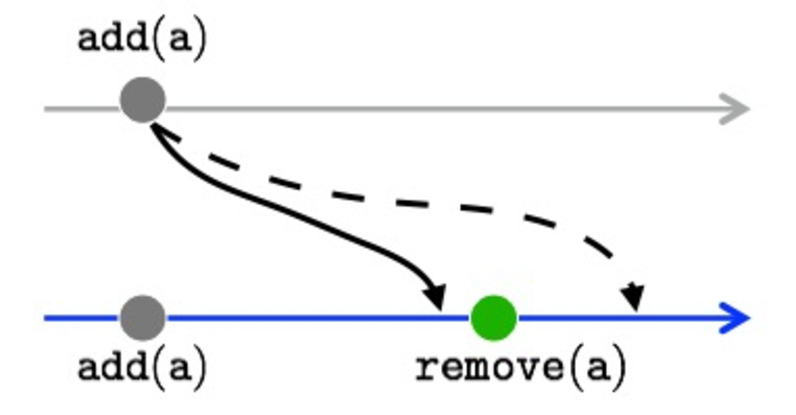
\includegraphics[width=0.35 \textwidth]{./figures/OR-Set-simple}
  \vspace{-5pt}
  \caption{Interleaving-based Set.}
  \vspace{-5pt}
  \label{fig:or-set-simple}
\end{wrapfigure}

\begin{figure}[!t]
  \centering
\begin{lstlisting}[caption={Pseudo-code of the OR-Set CRDT.},basicstyle=\ttfamily\scriptsize,captionpos=b,label={lst:or-set}]
  payload Set S
  initial S = @|$\emptyset$|@
  //@ initial lin = @|$\epsilon$|@

  add(a) :
    atSource :
      let k = getUniqueIdentifier()
      //@ lin = lin@|$\,\cdot\,$|@add(a,k)
    downStream(a, k) :
      S = S @|$\cup$|@ {(a, k)}
      //@ S' = S @|$\cup$|@ {(a, k)}

  remove(a) :
    atSource :
      let R = {(a,k) | (a,k) @|$\in$|@ S}
      //@ lin = lin@|$\,\cdot\,( $|@readIds(a)@|$\,\Rightarrow\,$|@R@|$ )\,\cdot\,$|@remove(a,R)
    downStream(R) :
      S = S @|$\setminus$|@ R
      //@ R == {(a,k) | @|$\exists\ \alabel$|@ = add(a,k). (@|$\alabel$|@, remove(a,R))@|$\in \avisord\ \land$|@
                              @|$ \forall\ \alabel'$|@ = remove(a,_). {(@|$\alabel,\alabel'$|@),(@|$\alabel'$|@, remove(a,R))}@|$\not\subseteq\,\avisord$|@}
      //@ S' = S @|$\setminus$|@ R

  read() :
    let A = {a : @|$\exists$|@ k. (a,k) @|$\in$|@ S}
    //@ lin = lin@|$\,\cdot\,$|@read@|$\,\Rightarrow\,$|@A
    return A
\end{lstlisting}
\end{figure}

<<<<<<< HEAD
=======
\begin{wrapfigure}{r}{.4\textwidth}
\vspace{-4mm}
  \centering
  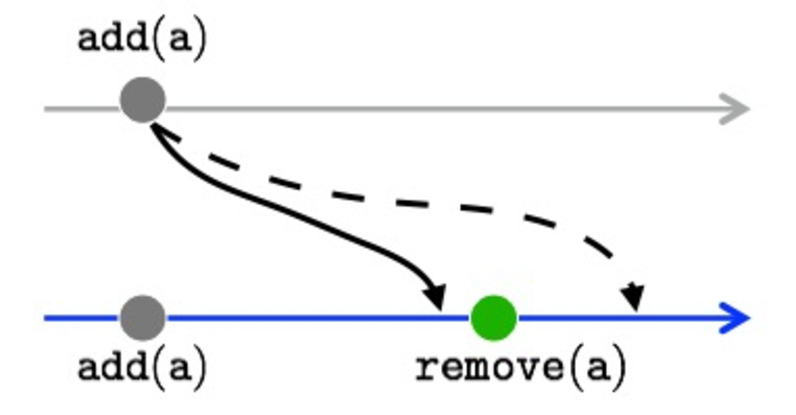
\includegraphics[width=0.35 \textwidth]{./figures/OR-Set-simple}
  \caption{Interleaving-based Set.}
  \label{fig:or-set-simple}
\end{wrapfigure}
>>>>>>> origin/master
The Observed-Remove Set (OR-Set)~\cite{ShapiroPBZ11} is another CRDT,
this time implementing a Set interface with methods: \lstinline|add(a)|,
\lstinline|remove(a)| and \lstinline|read()|.\footnote{Alternatively
  we could provide an interface with the method \lstinline|lookup(a)|
  returning a boolean with the same consequences as the
  \lstinline|read()|. This choice is of no consequence to our results.}
%

The meaning of these methods is self-evident from their names.
%
However, what is not evident is what are the results of conflicting
concurrent operations.
%
Consider for example the case where two replicas add a certain element
\lstinline|a| and then one of them removes that element.
%
If we consider an interleaving based execution of these operations
there are two options depending on the interleaving:
\begin{inparaenum}[i)]
\item If the \lstinline|remove(a)| operation is the last operation
  then the expected set is empty, since the two consecutive
  \lstinline|add(a)| operations are idempotent, and the
  \lstinline|remove| would remove the only occurrence of
  \lstinline|a|. This interleaving is the one depicted with solid
  arrows in Figure~\ref{fig:or-set-simple}.
\item On the other hand, if the operation \lstinline|add(a)| of the
  non-removing process comes last as depicted with the dashed arrows
  in Figure~\ref{fig:or-set-simple}, the final set could contain the
  element \lstinline|a|.
\end{inparaenum}
As we have explained before, in our system model the operations can
arrive in one order to one replica and in a different order to another
replica.
%
To guarantee convergence, OR-Set must ensure that regardless of the
ordering, the resulting set will be the same.
%
To that end, OR-Set \lstinline|add| operations will tag each added
element with a unique identifier.
%
Then, a remove operation will only remove the elements which has
already seen.
%
For instance, in the example above, the remove of \lstinline|a| will
only remove the element that has been previously added by the same
replica, since this item has been observed by the \lstinline|remove|
operation -- and thus its identifier is known to it --. However, the
concurrent \lstinline|add(a)| operation will have an identifier that
has not been observed by the \lstinline|remove| (since they are
concurrent).
%
Therefore the item will not be removed, even if the
effectors of the two adds are performed in a replica before the effector
of the remove.
%
The code of OR-Set is shown in Listing~\ref{lst:or-set} where for the time
being we ignore the lines marked with \lstinline|//@| annotations.

% \fxwarning[nomargin, inline]{If queries are discussed already for RGA,
%   here we should focus more on the rewriting of labels}
% \gpnote[nomargin, inline]{This is discussed just below, no?}

% \gpnote{Add reads at the end of the pictures.}

\begin{figure}[t]
  \begin{subfigure}{.9\linewidth}
    \centering
    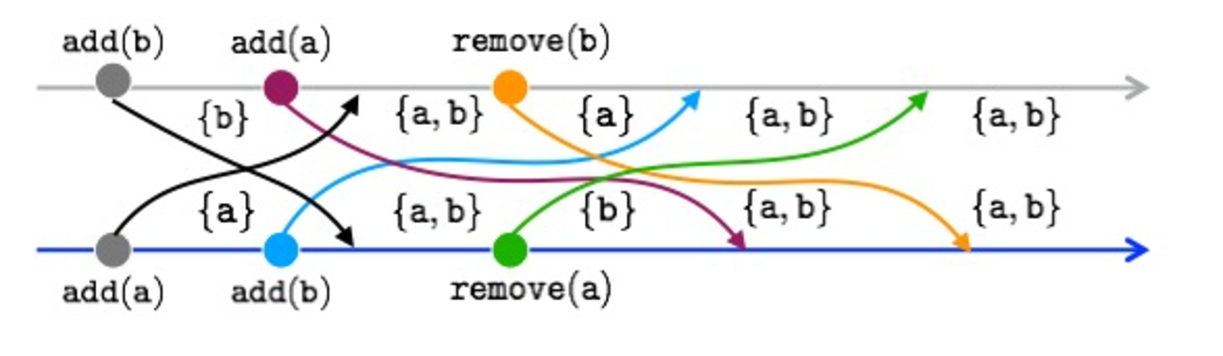
\includegraphics[width=0.70 \textwidth]{./figures/OR-Set-weird}
    \caption{OR-Set non-linearizable execution.}
    \label{fig:or-set-not-lin}
  \end{subfigure}
  \bigskip
  \bigskip

  \begin{subfigure}{.9\linewidth}
    \centering
    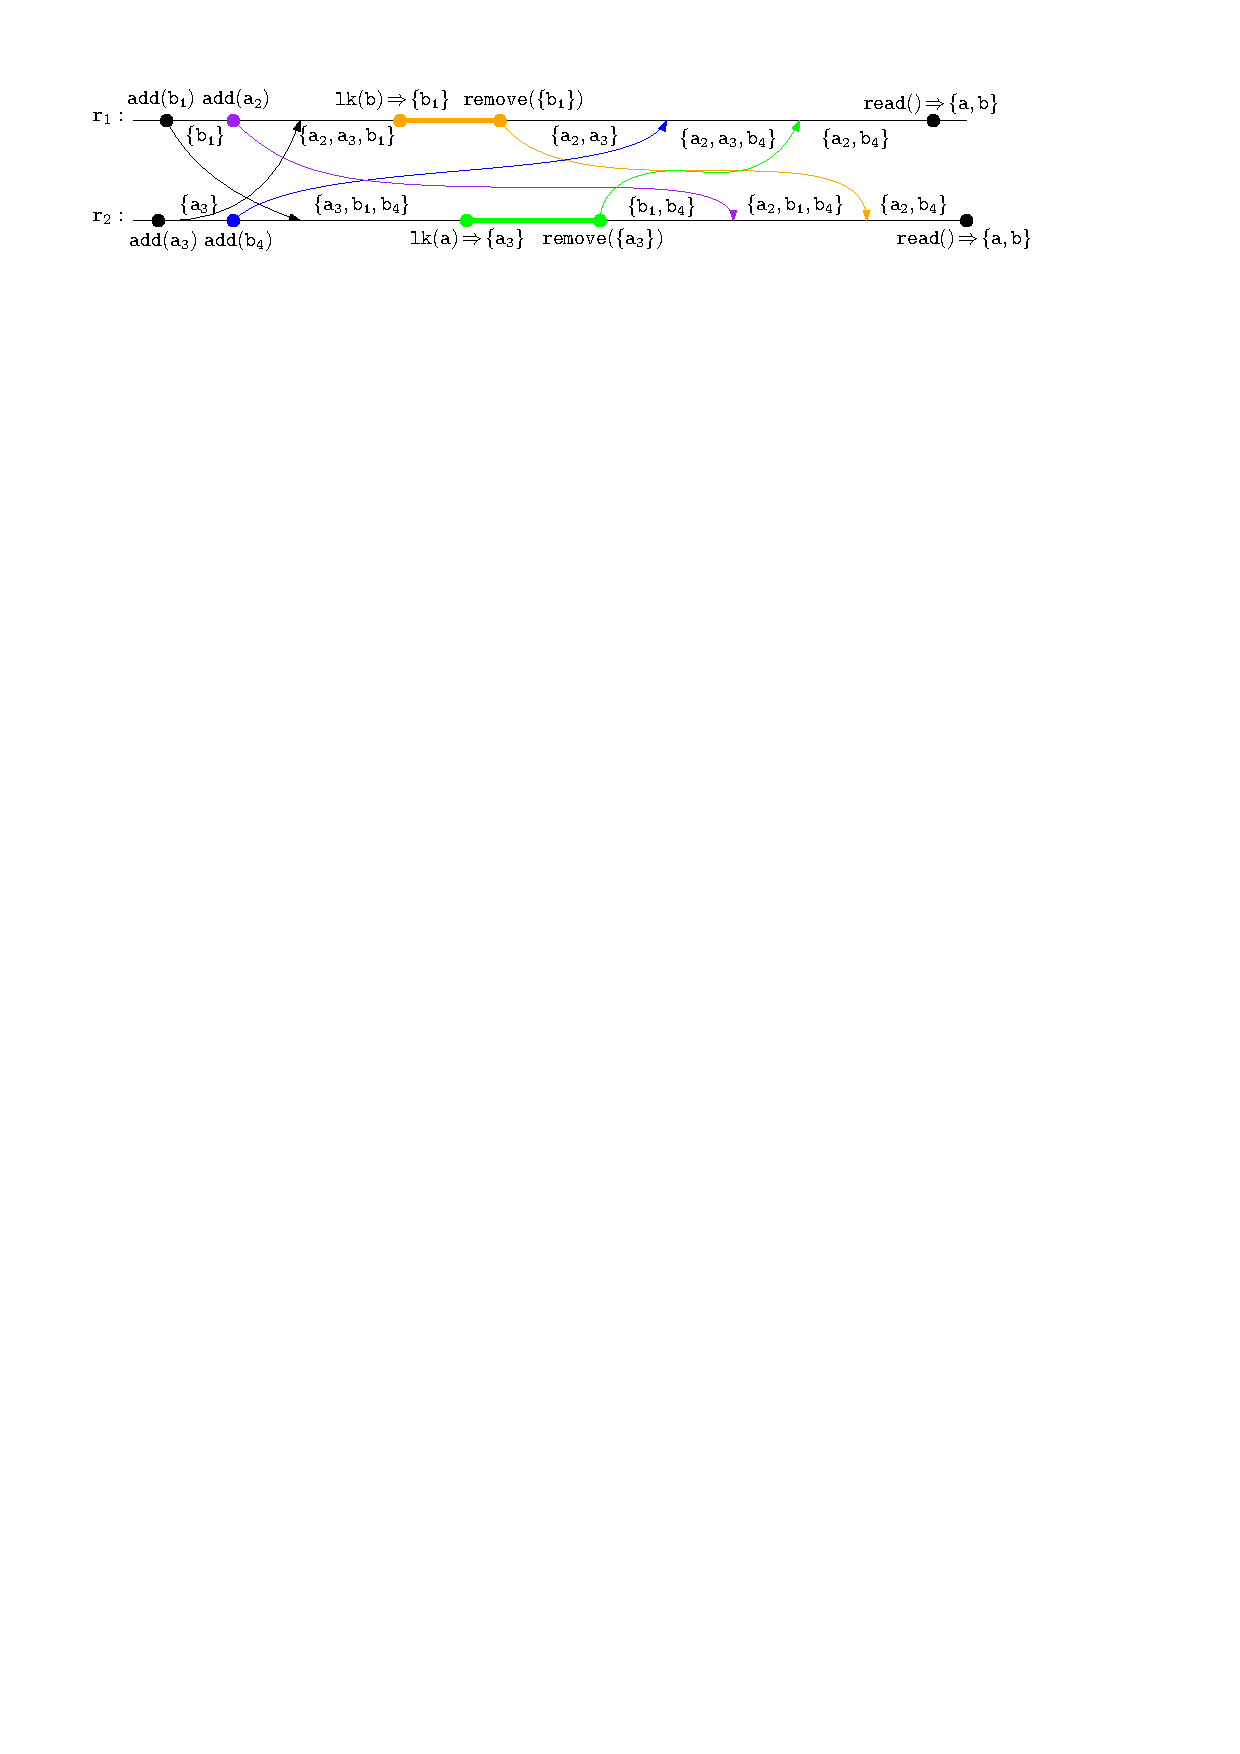
\includegraphics[width=0.95 \textwidth]{./figures/OR-Set-lk-rem}
    \caption{Label rewriting of an OR-Set execution.}
    \label{fig:or-set-lk-rem}
  \end{subfigure}
  \caption{OR-Set Linearizability vs. \CRDTLinshort{}.}
\end{figure}

\smallskip
\noindent
{\bf Intuition of OR-Set Linearizability.}
It is easy to find examples where the implementation of OR-Set can
produce executions which cannot be justified by standard definition of
linearizability (even with the relaxations discussed in Section~\ref{sec:rga-crdt-impl})
assuming a standard Set specification.
%
% \gpwarning{Redraw this picture properly.}
Figure~\ref{fig:or-set-not-lin} shows one such example.
%
For simplicity we assume here that we have two clients, each executing
in one of two replicas as their origin, issuing the sequences of
operations \lstinline|add(b);add(a);remove(b);read()| and
\lstinline|add(a);add(b);remove(a);read()| respectively.
%
The final reads are added only to exhibit the final state as perceived by
each replica through the API of the object.
%
Clearly any linearization of the visibility relation in this execution should order
the \lstinline|add| and \lstinline|remove| updates before the \lstinline|read| queries,
and the linearization of the updates should end with a
\lstinline|remove| operation. 
%Since the \lstinline|read| queries see all the updates
%in the execution, 
Therefore, the final set returned by each of the two \lstinline|read| queries should have
at most one element (note that the \lstinline|read| queries see all the updates
in the execution), contrary to their return value in this execution.
%that, in the final set we obtain:
%\{\lstinline|a, b|\} as observed by the result of the final
%\lstinline|read| operations.
%
% In other words, if in any of the replicas a \lstinline|read()|
% operation were to be issued, the result would be the set
% \{\lstinline|a, b|\} .

%For our definition of \CRDTLinshort{} we will distinguish between
%\emph{update} and \emph{query} operations.
%%
%We will impose two constraints, one on updates and another one on
%queries:
%\begin{itemize}
%\item For updates we require that there exists a total order of all
%  the updates in the execution -- essentially a linearization -- such
%  that the resulting state of the object -- or any intermediate state --
%  can be explained by executing the \emph{specification} of these
%  updates in order.
%%
%  Essentially, reachable states of the implementation are related to
%  specification states that can be reached by a certain global
%  linearization of the updates.
%%
%  \gpnote{Example?}
%\item Unfortunately, this simple requirement does not suffice for
%  query operations, since the system model allows for updates to arrive
%  to different replicas in different order.
%%
%  Hence, for \CRDTLinshort{} we will require that the result of any
%  query can be explained by consider a \emph{sub-sequence} of the above
%  mentioned global linearization of updates.
%\end{itemize}
%This definition will be made precise in~\autoref{sec:distributed-lin}.

%\gpnote{Maybe add a read example first?}
%To deal with this issue, we consider an additional relaxation of linearizability which 
%stems from the observation that 
%Coming back to our OR-Set example in~\autoref{fig:or-set-not-lin}, we
%have that 
This execution shows that 
the \lstinline|remove| operation behaves as both a query
(observing a certain number of adds of the element to be removed)
and an update (by removing said observed elements).
%
To cope with such cases, we will consider in our definition that
query-update operations can be split into a query part, which only
reads the state -- and hence is allowed to see a sub-sequence of the
linearization of updates --, and an update part which will use the
results of the prior query.
%
For instance, \lstinline|remove| will be split into a query part where
only the elements that are visible at the time of the remove are
selected, and an update part where only those elements selected are
erased.
%
Evidently, this requires some mechanism for ``marking'' the adds that
are concerned.
%
We will consider that each add has a unique identifier.
%
Then, the query part of a remove returns a set of unique identifiers
to be removed.
%
Any identifier not in this set will remain in the set after the update
part of the remove.
%
Figure~\ref{fig:or-set-lk-rem} shows this rewriting
where we denote by \lstinline|readIds| the query part of
remove, which returns a set of elements to be removed, and a
\lstinline|remove| operation taking a set of elements to be removed.
%
In this case, our definition of linearizability is just as before.
%
To linearize this execution, when contemplating only the updates, we
can chose any order consistent with the order in which operations are
performed in each replica and the result is consistent with the
specification of Set.
%
We discuss the details of this constructions in the next section.


% Method $\mathit{add}(a,b)$ intends to add item $a$ into the list at a
% position immediately after that of a existing item $b$. Method
% $\mathit{rem}(a)$ removes $a$ from the list. Method $\mathit{read}$
% returns the current list content. When the current replica does
% $\mathit{add}(a,b)$, it generate a tuple $(a,ts_a,ts_b)$ and put it
% into $N$. Here $ts_b$ is the time-stamp of $b$, and $ts_a$ is a new
% time-stamp that is larger than any time stamp in $N$. When the current
% replica does $\mathit{rem}(a)$, it put $a$ into tombstone. When the
% current replica does $\mathit{read}$, it uses function
% $\mathit{trans}(N,\mathit{Tomb})$ to return the list seen by the
% current replica, which is a sequences obtained by traversing $N$ in
% prefix order (children are visited in decreasing time-stamp order) and
% keeping only items that are not in $\mathit{Tomb}$.

%      precondition : %@|$\exists$|@ k. (a,k) @|$\in$|@ S
%let @|$\alabel = \alabellongind[remove]{a,R}{\bot}{i}$|@
%      //@ @|$\alpha(S) \xrightarrow{\alabelshort[add]{a,k}} \alpha(S')$|@
%       //@ @|$\alpha(S) \xrightarrow{\alabellongind[readIds]{a}{R}{}} \alpha(S)$|@
%       //@ @|$\alpha(S) \xrightarrow{\alabelshort[remove]{a,R}} \alpha(S')$|@
%     //@ @|$\alpha(S) \xrightarrow{\alabellongind[read]{}{A}{}} \alpha(S)$|@

% In the downstream of a $\alabellongNoret[\mathit{add}]{\argv}$
% operation, an tuple $(\argv,\ats)$ will be added to the local state;
% while in the downstream of a $\alabellongNoret[\mathit{add}]{\argv}$
% operation, a set $S_1$ will be removed from the local state. We call
% such tuple $(\argv,\ats)$ or set $S_1$ the content of the downstream.
% The following is the condition $C_2$ for or-set implementati.

%%% Local Variables:
%%% mode: latex
%%% TeX-master: "draft"
%%% End:
